\chapter{Experiments}
Now let us present a new approach, namely using the Scale-Invariant Model for network reconstruction. Where can this be useful? We saw, that the Scale-Invariant model describes networks consistently at different scales. Let us imagine a following situation: we want to study systemic risk in an interbank loan network. We know information about banks in the Czech Republic, therefore each of them can form a node in our network model, however, we have no information about banks in China, only their total exposure to Czech banks and vice versa. Therefore, China would only form one node. We clearly have two very different scales present in our network. Ordinary network models might handle this situation inaccurately, however the Scale-invariant model stays consistent even when there are multiple different scales present in the same network.

Let us formulate the problem in terms of interbank loan network. Assume we have $N$ banks labeled $1,\dots N$. We construct a liability matrix in the following way: if bank $i$ a lends money to bank $j$, then the amount lent will be the matrix entry $w_{ij}$. Thus, we obtain a weight-matrix $\hat{W}$ and a corresponding weighted directed graph. We denote the total amount lent by bank $i$ to all other banks (its assets) as $x_i \equiv \sum_{j=1} w_{ij} \equiv hat{s}^{out}$. We also denote the total amount which was lent \textit{to} bank $i$ (its liabilities) as $y_i \equiv \sum_{j=1}^N w_{ji} \equiv \hat{s}^{in}$. These total assets and liabilities are usually the only information disclosed publicly, while the details of the liability matrix are not known. 

\section{Network reconstruction using the original SIM}

Our approach will be similar as in the case of the Degree-corrected Gravity Model \ref{sec_DCGM}, but instead of the link probability from the fitness-induced DBCM model, we will use the Scale-invariant Model. Our approach is therefore as follows:

\begin{enumerate}
    \item We start with the information of the out-strengths $x_i \equiv s_0^{out}$ and in-strengths $y_i \equiv \hat{s}^{in}$ of each node (we call them \textbf{empirical strengths}) and the total number of links $\hat{L}$ (the subscript 0 denotes that it is a property of the original, empirical graph). 
    \item To use the Scale-invariant model, we need to estimate the value of $z$. For that, we demand the ensemble-average of the link-number to be equal to the number of links of the empirical network and find the corresponding $z$. The link probability between node $i$ and $j$ is for given $z$ 
    \begin{equation}
        p_{ij}^{SIM} = 1 - \exp(-z x_i y_j)
        \label{eq_prob_SIM}
    \end{equation}
    and thus we find the value of $z$ by solving the equation
    \begin{equation}
        \langle L \rangle = \mathbb{E}(\sum_{i,j=1}^{N} a_{ij}) = \sum_{i,j=1}^{N} p_{ij} = \sum_{i,j=1}^{N} (1 - \exp(-z x_i y_j)) \overset{!}{=} \hat{L}
        \label{eq:z_fit}
    \end{equation}
    \item We generate an ensemble of $M$ graphs, where $M$ is large enough. Usually, we generate 1000 graphs. Each graph is generated by sampling edges independently using the edge probability \ref{eq_prob_SIM} with corresponding strengths $x_i$, $y_j$ and $z$ from the previous step. When the graph is sampled, we assign weights to its edges in the same way as in the Degree-corrected Gravity Model, i.e.
    \begin{equation}
        w_{ij} = \begin{cases}
            0 \qquad &\text{if } a_{ij} = 0\\
            \frac{x_i y_j}{\tilde{W} p_{ij}^{SIM}} &\text{if } a_{ij} = 1
        \end{cases}    
    \end{equation}
    where $\tilde{W} \equiv \sum_{i=1}^N x_i =  \sum_{i=1}^N y_i$
    \item The generated ensemble is our reconstruction of the empirical network. If we know the empirical network, we can use it to determine the quality of our reconstruction. 
\end{enumerate}

We shall mention an important fact. The Scale-invariant model is proposed in such a way that it stays valid at any level of coarse-graining. However, that is not true for the way we assign weights in the point 3. When we coarse-grain, it is not equivalent to first assign weights to each edge and the sum the corresponding weights together vs. assigning weights at the coarse-grained level using the same formula. We would need to find a scale-invariant model for weighted graphs, which has been only tackled by one master's thesis yet \cite{Verteletskyi}.

\subsection{The dataset}
Our aim is to use this method in the networks of interbank loans. To evaluate the method, we would need to find a dataset with a full interbank loan network. Unfortunately, there is no such dataset freely available. Therefore, we need to find a dataset similar enough. 

For our purposes, we will use the US Airport Network. The dataset contains data for 25 years (1990-2015) of flights between cities in the US\footnote{More information about the dataset can be found at \href{https://ericmjl.github.io/Network-Analysis-Made-Simple/05-casestudies/02-airport/}{https://ericmjl.github.io/Network-Analysis-Made-Simple/05-casestudies/02-airport/}}. If there is a connection between those two cities, the dataset contains the number of passengers taking that connection in a given year. 

Therefore, we can construct a graph, where vertices are airports, edge is present if there is a connection between two different airports and the edge weights are the numbers of passengers on that route. By that, we obtain a directed weighted graph. 

Such a dataset might be similar to the interbank loan network. There is a wide heterogeneity in the size of airports, same as the size of banks. On the other hand, in the airport network, we expect a high reciprocity - if there is a link between A and B with some number of passengers, there is probably a link from B to A with a similar number of passengers. That might not be the case in the interbank networks, as we do not necessarily expect each loan to be reciprocated (actually, we expect the opposite). 

Let us take only the data from the year 2015. We only take those airports which have at least one out-coming and one in-coming connection (non-zero out- and in-strength). In such case, we obtain a network with 1021 vertices and $19\mathpunct{}199$ edges. The number of all possible edges (pairs of nodes) is $1\mathpunct{}042\mathpunct{}441$, therefore our network can be still considered sparse. 

Figure \ref*{fig:deg_strengths} shows the log-log plots of degree and strength distributions. We can see that the out-degree distribution might be fitted by a power-law (straight line in the log-log plot). Gabrielli et al. \cite{Gabrielli2024} study an empirical interbank dataset and find a good fit of the strength distribution using a log-normal distribution. On our plot, however, we can see that although the distribution is decaying fast for high strengths, low strengths do not decay fast enough for the distribution to be log-normal. We could propose to only take vertices with strengths higher than some threshold, but for further purposes we will keep the original data.

\begin{figure}[!ht]
    \centering
    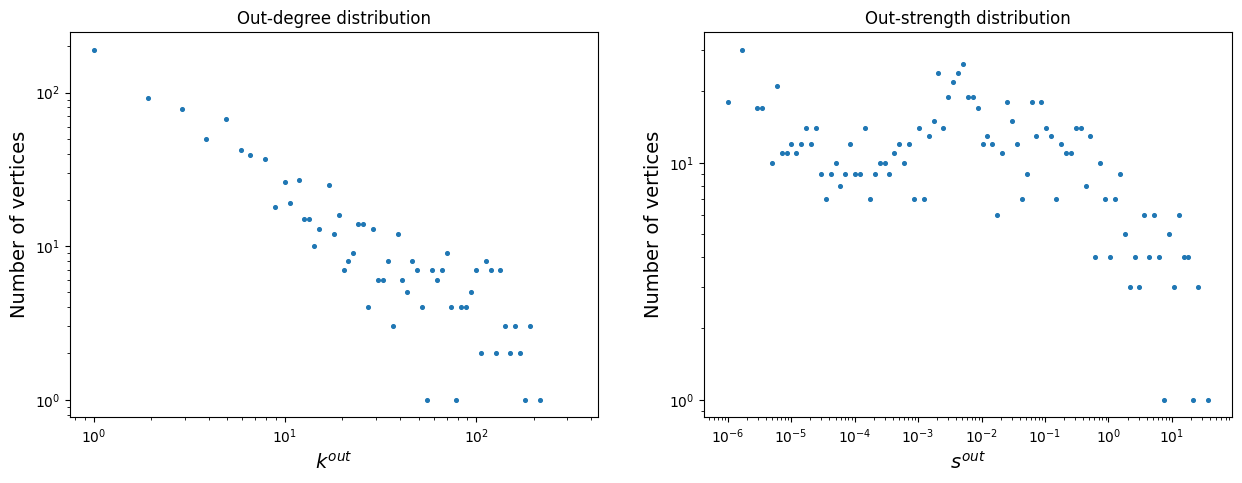
\includegraphics[scale=0.5]{../img/vanilla_SIM/deg_strengths.png}
    \caption{Out-degree and out-strength histograms for the airport network.}
    \label{fig:deg_strengths}
\end{figure}

\subsection{Reconstruction}
Now we can follow the recipe shown above. First, we need to find the value of $z$, that will reproduce the number of links correctly. We solve the equation \ref{eq:z_fit} using bisection method. To avoid numerical problems, we divide all strengths by $10^6$, since the largest strength in our dataset is $44\mathpunct{}337\mathpunct{}603$. By that, we obtained $z \doteq 0.2837$.

Next, we generate an ensemble of 1000 graphs using the Scale-invariant model. The first consistency check is to find the average number of links in our ensemble. That is, for our ensemble, $19\mathpunct{}198.329$, which is close enough to the $19\mathpunct{}199$ edges of the original ensemble.

Next, we can compare properties of the empirical graph and our ensemble. For directed properties (like strengths: out-strengths and in-strengths), we will always show the out-properties, as we did not observe significant difference between the directions.

\subsubsection{Degrees and strengths}
The question of network reconstruction is: can we reproduce the properties of the empirical network by our ensemble on average? This needs to be shown by comparison. Let us first compare these properties node by node. For each node, we can compute the desired property in the empirical graph and also in each graph in the ensemble. Then, for each node, we average its property over the ensemble. 

Figure \ref*{fig:deg_strengths_rec} shows the comparison of empirical degrees and strengths. We can see that strengths are reconstructed very well over the ensemble. Only for nodes, which have low strength in the original ensemble, the reconstruction gets worse, but that is probably due to the limited size of the ensemble. On the other hand, we can see that the degrees are reconstructed on average well only in the high-strength regime. For lower strengths, we see that ensemble averages get below 1, but the degrees in the empirical ensemble are never below one, since there are no isolated nodes.

\begin{figure}[!ht]
    \centering
    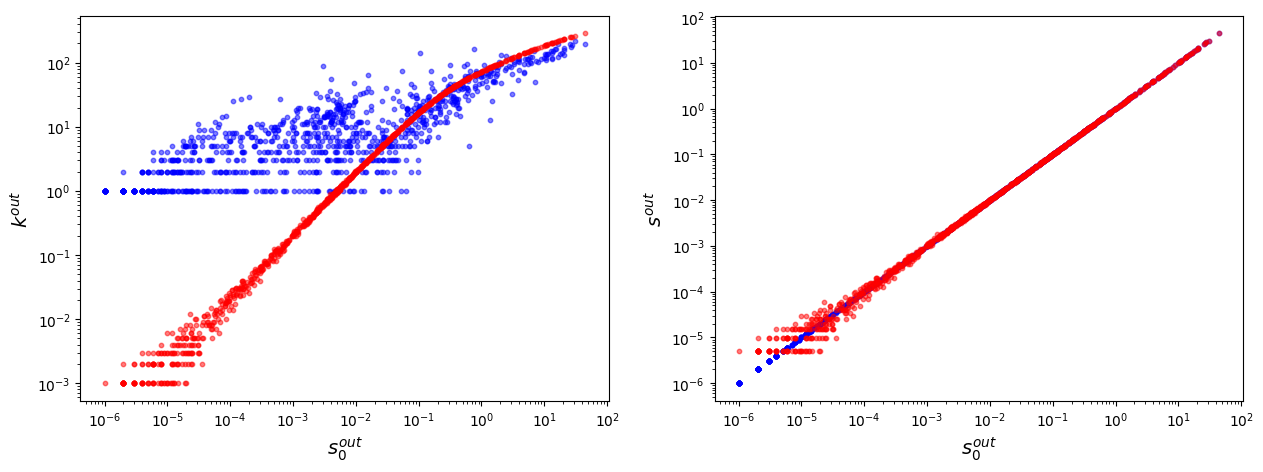
\includegraphics[scale=0.5]{../img/vanilla_SIM/deg_strengths_rec.png}
    \caption{Comparison of out-degrees and out-strengths. Blue points are nodes in the original ensemble, red points are averages of degrees or strengths over the ensemble for each node. Properties are compared against the $s_0^{out}$, the empirical out-strengths (strengths from the empirical ensemble).}
    \label{fig:deg_strengths_rec}
\end{figure}

One can also compare the degree and strength histograms. For each network in the ensemble, we can compute its own degree and strength histogram, and then average them. The result can be found on figure \ref*{fig:deg_strengths_hist_rec}. We can observe two interesting phenomena. First, the model reproduces the degree distribution considerably well, however, it generates certain number of nodes with much higher degree, than what was observed in the empirical graph and underestimates the number of low-degree nodes on the other hand. Second, the strength distributions in the ensemble do not show any nodes with strengths lower than $10^{-3}$, however the strengths in the empirical graph go as low as $10^{-6}$. This can be also probably ascribed to the absence of isolated nodes in the empirical graph. The nodes with low empirical strengths end up being isolated in reconstructed graphs, therefore having zero strength.

\begin{figure}[!ht]
    \centering
    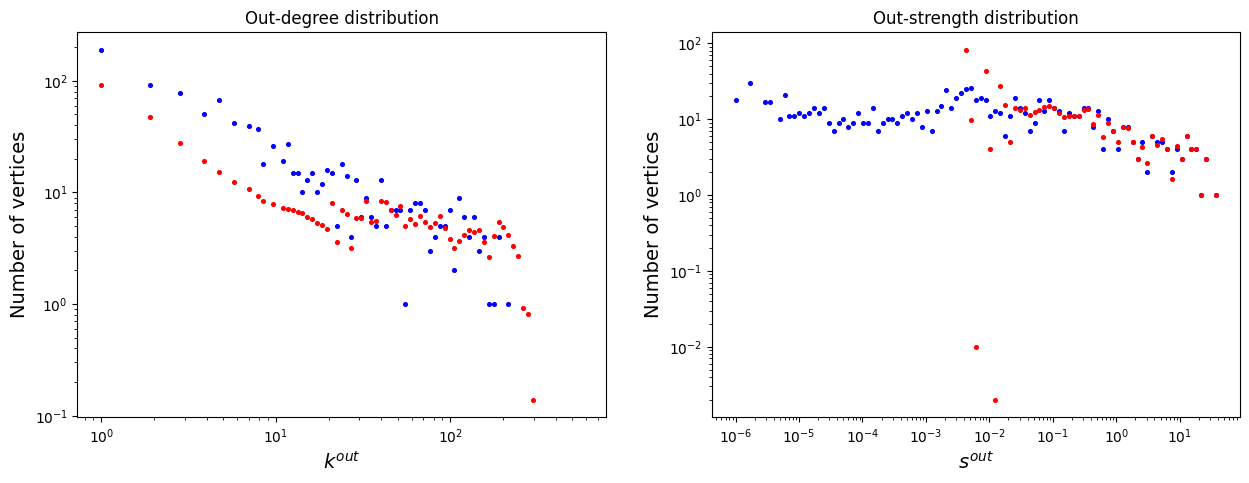
\includegraphics[scale=0.5]{../img/vanilla_SIM/deg_strengths_hist_rec.png}
    \caption{Comparison of degree histograms for the empirical network (blue) and the reconstructed ensemble (red). We can observe that our method produces nodes with higher degrees than what are present in the empirical network. On the other hand, it does not produce nodes with strengths lower than $10^{-3}$.}
    \label{fig:deg_strengths_hist_rec}
\end{figure}

\subsubsection{Average nearest-neighbor degree and local clustering coefficient}
Since we assigned strengths in a way to reconstruct them well on average, we should not be surprised, that they actually were reproduced quite well. The more interesting thing is to study higher order properties like average nearest-neighbor degree or local clustering coefficient. If these can be reproduced well, we have a sign that our reconstruction method works well. 

On figure \ref*{fig:ANND_ANNS}, we can see the comparison of average nearest-neighbor degree (ANND) and average nearest-neighbor strength for each node. We can see that ANND approaches good reconstruction for nodes with high empirical strengths, but for the rest of the nodes, ANND is mostly overestimated. This can be connected with the problem we saw on the histogram \ref*{fig:deg_strengths_hist_rec}, that low degree nodes are underestimated and there are some nodes in the reconstructed ensemble with significantly higher degrees than in the empirical graph.

\begin{figure}[!ht]
    \centering
    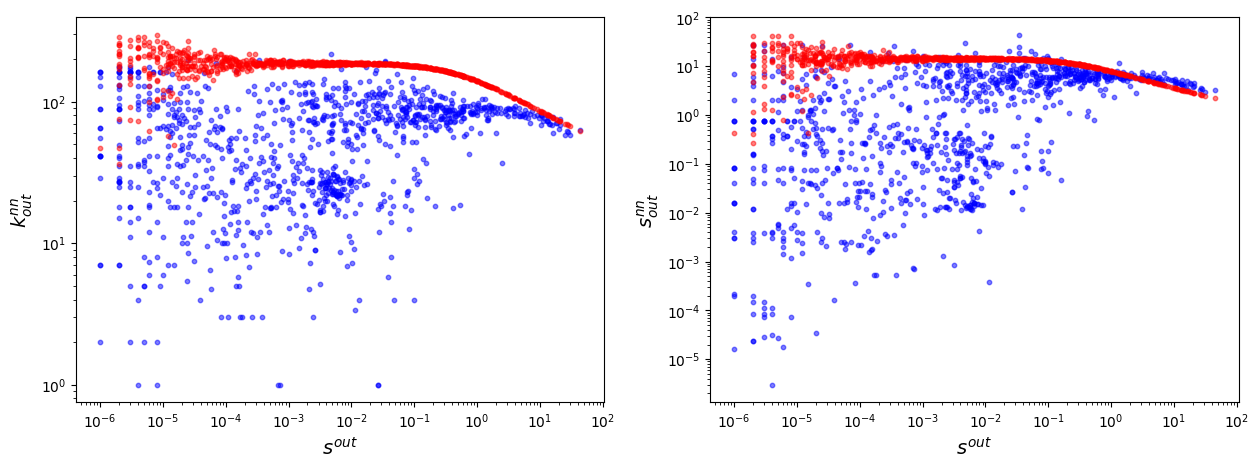
\includegraphics[scale=0.5]{../img/vanilla_SIM/ANND_ANNS.png}
    \caption{Comparison of ANND and ANNS for the empirical graph (blue) and the reconstructed ensemble (red). On the x-axis, there are the empirical strengths.}
    \label{fig:ANND_ANNS}
\end{figure}

Another comparison which is done in the field of network reconstruction, is aggregating nodes with the same degree in groups and for each group computing the average of some property, for example ANND or the local clustering coefficient. We can see such comparison for the ANND on figure \ref*{fig:ANND_k}. Here the overestimation of ANND is even more pronounced. ON the other hand, disassortative tendency (high-degree nodes have on average lower degree neighbors) is reconstructed well.

\begin{figure}[!ht]
    \centering
    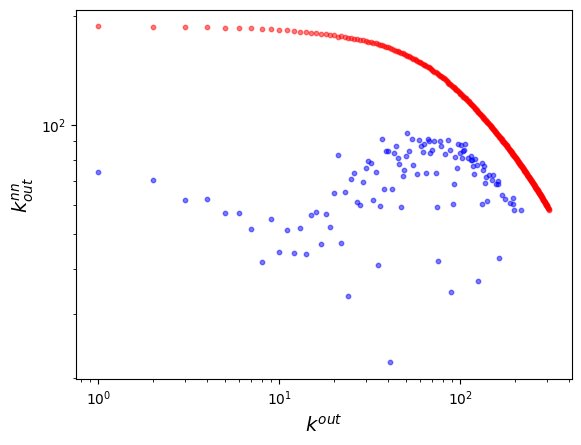
\includegraphics[scale=0.5]{../img/vanilla_SIM/ANND_k.png}
    \caption{Comparison of ANND and ANNS for the empirical graph (blue) and the reconstructed ensemble (red). On the x-axis, there are the empirical strengths.}
    \label{fig:ANND_k}
\end{figure}

We may compare local clustering coefficient as well (see figure \ref*{fig:cl_coeff}). Similarly to ANND, the decreasing tendency of the clustering coefficient is reconstructed well and also the nodes with high empirical-strength show a good correspondence. On the other hand, lower strength nodes have usually higher ensemble-average clustering coefficient than in the empirical graph.

\begin{figure}[!ht]
    \centering
    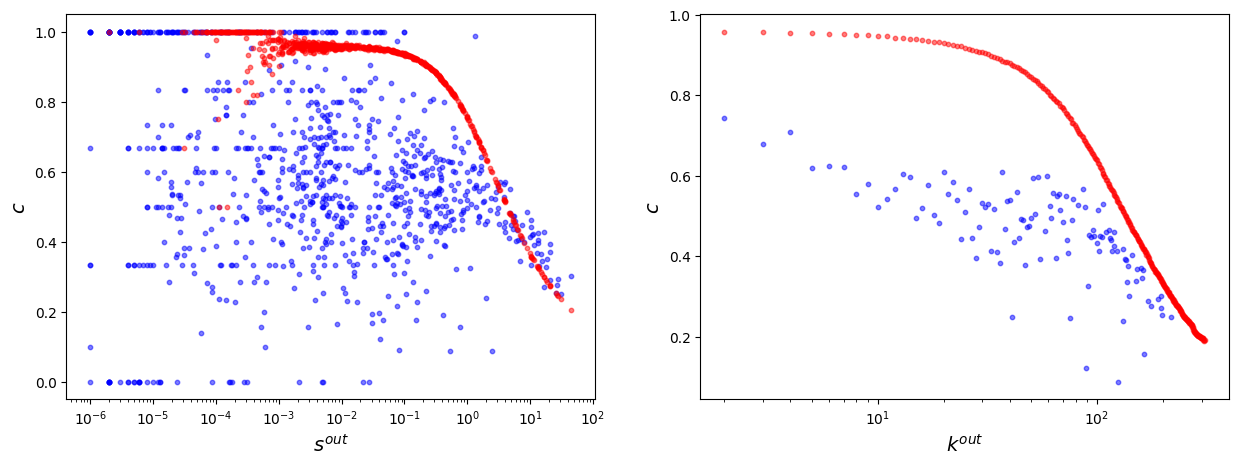
\includegraphics[scale=0.5]{../img/vanilla_SIM/cl_coeff.png}
    \caption{Comparison of the local clustering coefficient for the empirical graph (blue) and the reconstructed ensemble (red). The graph on the left compares each node depending on its empirical strength. The graph on the right shows the aggregated local clustering coefficient for each node degree.}
    \label{fig:cl_coeff}
\end{figure}


\subsubsection{Isolated nodes}
Since we observed, that isolated nodes can pose a problem in the network reconstruction, let us compute, how many of them are there in the reconstructed networks. Let us remind, that the empirical graph has zero isolated nodes, each node has at least one out-going link and one in-going link.

We computed average numbers of out-isolated nodes (nodes with no out-going links) and in-isolated nodes (nodes with no in-going links). Out of 1021 nodes, there were on average 502.745 out-isolated nodes and 503.166 in-isolated nodes. This is remarkably \textbf{bad} result for the financial network reconstruction. 

\section{Degree corrected SIM}
The problem of isolated nodes is actually a crucial one in the financial network analysis. Usually, we want to study dynamical processes, where some signal spreads through the network. For example, the DebtRank model \cite{Bardoscia2015} studies, how the stress spreads in the network when some bank loses a significant portion of its equity. In some cases, the network can dissipate such stress, but also a big bank crisis can occur. If our reconstruction method generates isolated nodes, these do not take part in the stress propagation and our analysis can not be valid. 

We saw that we can not stick to the original model, if we want to avoid too many isolated nodes. Therefore, we want to find such an extension of the scale-invariant model, which imposes some additional constraints while still keeping the scale-invariant properties.

How to extend the SIM in the most ``minimal'' way? We can sample from the original SIM, but then throw away those realizations, which contain isolated nodes. This seems trivial, however generating even one such sample could be very much time-consuming. We thus need to find a more clever sampling strategy.

\subsection{The naive approach}
Let us assume, that every node has out-degree greater or equal than 1, while we do not have requirements on in-degrees (the opposite situation - nonzero in-degrees and no requirements for out-degrees - could be considered analogously). How are the connection probabilities influenced by that assumption?

\begin{equation}
    P(a_{ij}=1|k_i^{out}\geq 1) = \frac{P(a_{ij}=1 \cap k_i^{out}\geq 1)}{P(k_i^{out}\geq 1)} = \frac{P(a_{ij}=1)}{P(k_i^{out}\geq 1)}
\end{equation}

Now, we need to find $P(k_i^{out}\geq 1)$. Let the self-loops contribute to the degree for simplicity.
\begin{align}
    P(k_i^{out}\geq 1) &= 1-P(k_i^{out}=0) = 1 - \prod_j(1-p_{ij}) = 1 - \prod_j\exp(-zx_i y_j) \\
    &= 1 - \exp(-zx_i\sum_j y_j) = 1 - \exp(-zx_i W)
\end{align}

Therefore
\begin{equation}
    P(a_{ij}=1|k_i^{out}\geq 1) = \frac{P(a_{ij}=1)}{1 - \exp(-zx_i W)} = \frac{1-\exp(-zx_iy_j)}{1 - \exp(-zx_i W)}
    \label{eq:posterior_proba}
\end{equation}

Let us examine, what we achieved. For $x_i$ large, $\exp(-z x_i W) \to 0$ and the effect of our correction is negligible. However, when $x_i$ is small, the denominator starts to play a role and increases connection probability, so it is more probable to have at least one connection. 

Now we could just use these connection probabilities instead of those from the original SIM. However, we call this the naive approach, because it has one significant flaw. If we sample each edge $a_{ij}$ independently, the probability $P(k_i^{out}=0)$ is nonzero, since

\begin{align}
    P(k_i^{out}=0) &= P(a_{ij}=0, \forall j) = \left\{ \text{independent sampling} \right\} = \\ &= \prod_{j} P(a_{ij}=0|k_i^{out}\geq 1) = \frac{\exp(-zx_iy_j)}{1 - \exp(-zx_i W)} > 0
\end{align}

This means that such a model could still produce isolated nodes.

In table \ref*{table:comparison_1}, we can see several results of the naive model compared to the original SIM. The number of out-isolated nodes was decreased significantly, however, as we explained, it is not zero. Also, the number of in-isolated nodes remained unchanged. We can observe one interesting phenomenon - the number of edges increased. This is due to the fact, that we used the same value of $z$ as in the original SIM. Since this model has a tendency to create more edges, we need to find a corresponding value of $z$, which will be lower than in the original model. We will tackle this problem in the following paragraphs.

\subsection{Correction the naive model - Out-degree corrected SIM}

The problem with the naive approach above is, that since we added the requirement of nonzero degree, we introduced dependence among edges. To be precise, if we demand $k_i^{out}\geq 1$, we make the random variables ${a_{ij}}$ dependent, i.e. the $i$-th row of the adjacency matrix is dependent. To actually sample from the conditioned distribution, we need to sample the rows of the adjacency matrix at once.

The conditional probability of the $i$-th row (which we denote $\{a_{ij}\}_{j=1}^N$) can be found:
\begin{align}
    P\left(\{a_{ij}\}_{j=1}^N|k_i^{out}\geq 1\right)
    &= \frac{P\left(\{a_{ij}\}_{j=1}^N\right)}{P(k_i^{out}\geq 1)} = \frac{ \prod_{j=1}^N P_{ij}^{a_{ij}}(1-P_{ij})^{(1-a_{ij})} }{P(k_i^{out}\geq 1)} \\
    &= \frac{ \prod_{j=1}^N (1 - \exp(-z x_i y_j))^{a_{ij}}\exp(-z x_i y_j)^{(1-a_{ij})} }{1 - \exp(-zx_i W)}
    \label{eq:corrected_naive_model}
\end{align}

How to implement sampling? In our case, it proved to be computationally feasible to sample each row as a whole from the original model and only accept it, when the condition of at least one present edge is met. This is equivalent to sampling according to the conditional probabilities given by equation \ref*{eq:corrected_naive_model}. 

Another flaw of the naive model is that we used the original value of $z$, which is, however, not valid anymore. The value of $z$ need to fit the density (or number of edges) of the empirical network, so if we change the model, we need to find an according value of $z$. This can be done analytically. In equation \ref*{eq:corrected_naive_model}, we see that the difference with the original SIM is in the denominator. The expected number of links in each row will be therefore be, compared to the original model, increased due to the division by this denominator. 




\subsubsection{Results}
First we plot the average strengths vs. the empirical ones. One can see that on figure \ref*{fig:degrees_strengths_rec_corrected_naive}. The out-strengths are reproduced perfectly and out-degrees have no longer problem with averages lower than one. On the other hand, the figure also shows the in-degrees and in-strengths, whose properties did not change compared to the original SIM.

\begin{figure}[!ht]
    \centering
    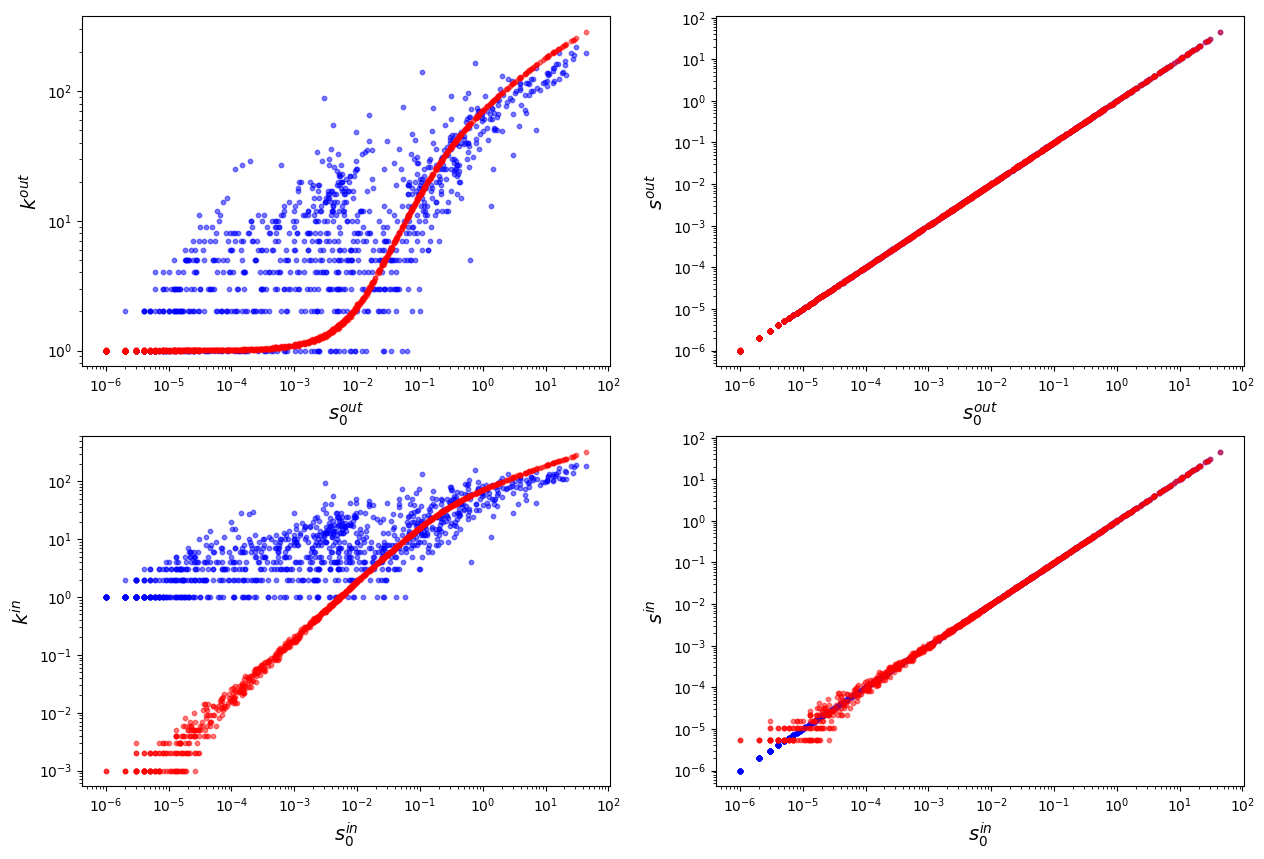
\includegraphics[scale=0.5]{../img/corrected_naive/degrees_strengths_rec.png}
    \caption{Comparison of both out-degrees, out-strengths and in-degrees, in-strengths. Blue points are nodes in the original ensemble, red points are averages of degrees or strengths over the ensemble for each node. Properties are compared against the $s_0^{out}$, the empirical out-strengths (strengths from the empirical ensemble).}
    \label{fig:degrees_strengths_rec_corrected_naive}
\end{figure}

In table \ref*{table:comparison_1}, we can see other results. Since we fitted $z$ specifically for the corrected model, we can see that the number of edges is again close to the one of the empirical graph. The number of out-isolated nodes is finally 0, on the other hand, the average number of in-isolated nodes even slightly increased. Also, the average maximum degree is higher than in the original model and significantly higher than in the empirical graph.

\begin{table}
\centering
\begin{tabular}{ |p{3cm}||p{2cm}|p{2cm}|p{2cm}|p{2cm}|  }
 \hline
 \multicolumn{4}{|c|}{Properties} \\
 \hline
 Property & Empirical network & SIM & Naive approach & Out-degree corrected SIM \\
 \hline
 Number of out-isolated nodes   & 0    &502.745&   200.101 & 0\\
 Number of in-isolated nodes   & 0    &503.166&   502.384 & 508.548\\
 Number of edges&   19199  & 19198.329  &19759.582 & 19195.15\\
 Maximal degree & 408 & 576.953&  611.876 & 602.796\\
 \hline
\end{tabular}
\caption{Comparison of the empirical network, original Scale-invariant model and its naive and corrected modifications.}
\label{table:comparison_1}
\end{table}

We can see that the number of isolated nodes decreased significantly, but they still form a fraction, which is not negligible.

\subsection{Correction of out-degrees and in-degrees simultaneously - Degree corrected SIM}
In the previous approach, we used the fact that we can sample out-links of each node independently. That was possible because we demanded only out-degrees to be nonzero. If we demand out-degrees and in-degrees to be nonzero simultaneously, we obtain dependence through the whole set of links, and we need to sample the whole graph at once.

The conditional probability of the whole graph configuration (which we denote $\{a_{ij}\}_{i,j=1}^N$) looks as follows

\begin{equation}
    P\left(\{a_{ij}\}_{i,j=1}^N \, | \, (k_i^{out} > 0 \, \forall i) \cap (k_i^{in} > 0 \, \forall i )\right) = \frac{P\left(\{a_{ij}\}_{i,j=1}^N \cap (k_i^{out} > 0 \forall i) \cap (k_i^{in} > 0 \forall i )\right)}{P\left((k_i^{out} > 0 \, \forall i) \cap (k_i^{in} > 0 \, \forall i )\right)}
\end{equation}

A configuration, which does not satisfy the conditions has zero probability. Let us denote the space of all possible graphs with $(k_i^{out} > 0 \, \forall i) \cap (k_i^{in} > 0 \, \forall i )$ as $\Gamma$. Then on this space, we can define a new random graph model given by graph probability $P_\Gamma$:
\begin{equation}
    P_\Gamma\left(\{a_{ij}\}_{i,j=1}^N\right) = \frac{P\left(\{a_{ij}\}_{i,j=1}^N\right)}{P\left((k_i^{out} > 0 \, \forall i) \cap (k_i^{in} > 0 \, \forall i )\right)} \qquad \forall \{a_{ij}\}_{i,j=1}^N \in \Gamma
\end{equation}
where $P$ is the probability induced by the original Scale-invariant model. 

The denominator (normalization constant, partition function) is difficult to compute. Also, if we could obtain probabilities for all configurations $\{a_{ij}\}_{i,j=1}^N$, it would still be usually hard to sample directly from the distribution obtained. We would have to sample the whole graph at once, and if the number of allowed configurations is high, each probability can be very low, and we could encounter numerical problems.

To avoid these obstacles, we propose to use the Metropolis-Hastings algorithm. The main advantage of it is that we do not to know the normalization function (partition sum) explicitly, as it only uses the ratio of probabilities.

We will proceed in the following manner:

\begin{enumerate}
\item We start from any configuration complying to our conditions. For example, we can connect node 1 to 2, 2 to 3 and so on to form a circle. Then we can add additional edges to have a similar number of edges as in the empirical graph.
\item We propose a new configuration by flipping any entry $a_{ij}$ of the adjacency matrix from 1 to 0 or from 0 to 1. We choose such entry uniformly randomly.
\item If the proposal does not comply to our condition, we refuse it and randomly choose entry $a_{ij}$ again. We do that until we obtain an allowed configuration.
\item Having an allowed proposal, we calculate the acceptance ratio. Since we flipped only entry $a_{ij}$, the ratio of probabilities of the proposal vs. the initial graph is $\alpha = \frac{p_{ij}}{1-p_{ij}}$ if the proposed $a_{ij} = 1$ or $\alpha = \frac{1-p_{ij}}{p_{ij}}$ if proposed $a_{ij} = 0$
\item We generate a uniform number $u \in [0,1]$. If $u\leq\alpha$, we accept the proposal, otherwise we keep the adjacency matrix from the previous step. Then we repeat the algorithm from step 2).
\end{enumerate}

The disadvantage of this approach is that we get highly autocorrelated series of graphs. Therefore, we can only choose each $i$-th graph from this procedure (this method is usually called thinning). The higher the $i$ is, the less autocorrelated ensemble we get. 

Also, it takes some time for the algorithm to reach the high-probability region, therefore we implement the so-called burn-in period, which means we discard the first $j$ samples.

\subsubsection{Finding a proper value of $z$}
This corrected model still depends on the value of $z$. We can not choose the same value of $z$ as in the original model, since we reject unplausible realizations of it and therefore our correction naturally increases the number of links compared to the original model. We need to fit $z$ according to the empirical network we have.

In this sense, we fit $z^*$ in such a way to replicate the number of links well. In the original SIM, we demanded
\begin{equation}
    L_0 = \langle L \rangle = \sum_{i,j} p_{ij} = \sum_{i,j} P(a_{ij} = 1) = \sum_{i,j} 1-\exp{(-z^*x_iy_j)}
\end{equation}
In the corrected model, things get more complicated. 
Let us first denote the marginal probability (denoted as $p_{ij}^M$) of every edge $a_{ij}$ as
\begin{equation}
    p_{ij}^M = \sum_{\{a_{kl}\} \in \Gamma, a_{ij} = 1} P_\Gamma\left(\{a_{ij}\}_{i,j=1}^N\right)
\end{equation}
i.e. we are summing probabilities of all possible configurations from $\Gamma$ where $a_{ij} = 1$. 

Then we get
\begin{align}
    \langle L \rangle &= \mathbb{E}_\Gamma\left(L\right) = \mathbb{E}_\Gamma\left(\sum_{i,j=1}^{N} a_{ij}\right) = \sum_{\{a_{kl}\} \in \Gamma} \sum_{i,j=1}^{N} a_{ij} P_\Gamma\left(\{a_{kl}\}\right) = \sum_{i,j=1}^{N} \sum_{\{a_{kl}\} \in \Gamma} a_{ij} P_\Gamma\left(\{a_{kl}\}\right)\\
    =&  \sum_{i,j=1}^{N} \sum_{\{a_{kl}\} \in \Gamma} a_{ij} P_\Gamma\left(\{a_{kl}\}\right) = \text{\{the case $a_{ij} = 0$ does not contribute\}} = \\
    =& \sum_{i,j=1}^{N} \sum_{\{a_{kl}\} \in \Gamma, a_{ij} = 1} P_\Gamma\left(\{a_{ij}\}_{i,j=1}^N\right) = \sum_{i,j=1}^{N} p_{ij}^M
\end{align}
which means, that instead of the probabilities from the original model, we should use marginal probabilities induced from our corrected model. However, the marginal probabilities are difficult to compute analytically. 

As an approximative workaround, we can find the value of $z^*$ by bisection on simulations. Since the number of links is on average increasing function of $z$, we can start with some guess, generate a corresponding ensemble, compute the average number of links, and if it's higher than the demanded number of links of the empirical network, we know we need to decrease $z$. Otherwise,x we increase it. Therefore, we can find value of $z^*$ using bisection to a demanded precision. The precision is not arbitrary, however, since there is a estimation error present, as we only estimate the number of links on the generated ensemble.

\subsubsection{Assigning weights}
The question remains, how to assign weights in this case. Our original model does it in the following way:
\begin{equation}
    w_{ij} = \frac{x_iy_j}{Wp_{ij}}
\end{equation}
where $p_{ij} = P(a_{ij} = 1)$. How do we replace $p_{ij}$?

Let us assume the weights are of form $w_{ij} = w(x_i, y_j)a_{ij}$. Then the expected out-strength of node $i$ in an ensemble is

\begin{align}
    \langle s_i^{out} \rangle &= \mathbb{E}_\Gamma\left(\sum_{j=1}^{N} w_{ij}\right) = \sum_{\{a_{kl}\} \in \Gamma} \sum_{j=1}^{N} w_{ij} P_\Gamma\left(\{a_{kl}\}\right) = \sum_{j=1}^{N} \sum_{\{a_{kl}\} \in \Gamma} w_{ij} P_\Gamma\left(\{a_{kl}\}\right) \\ &= \sum_{j=1}^{N} \sum_{\{a_{kl}\} \in \Gamma} w(x_i, y_j)a_{ij} P_\Gamma\left(\{a_{kl}\}\right) \\ &= \text{\{the case $a_{ij} = 0$ does not contribute\}} \notag \\
    &= \sum_{j=1}^{N} w(x_i, y_j) \sum_{\{a_{kl}\} \in \Gamma, a_{ij} = 1} P_\Gamma\left(\{a_{ij}\}_{i,j=1}^N\right) \\
    &= \sum_{j=1}^{N} w(x_i, y_j) p_{ij}^M
\end{align}

Therefore, we just need to assign $w(x_i, y_j) = \frac{x_i y_j}{W p_{ij}^M}$, because then
\begin{equation}
    \langle s_i^{out} \rangle = \sum_{j=1}^{N} w(x_i, y_j) p_{ij}^M = \sum_{j=1}^{N} \frac{x_i y_j}{W p_{ij}^M} p_{ij}^M = x_i \frac{\sum_{j=1}^{N} y_j}{W} = x_i
\end{equation}
which means we obtain the correct out-strength $x_i$ on average. This means we only need to obtain the marginal probabilities for each link to assign weights. As we know from estimation of $z$, we know it is hard to compute this probability analytically. However, we can estimate it as well. 

We generate an ensemble using our corrected model. This yields an ensemble of average matrices, from which we can compute an average adjacency matrix. Entries of this average adjacency matrix can be used as estimates of the marginal probabilities.

\subsubsection{Results}
We used the Metropolis-Hastings algorithm as explained above. The first configuration we use is the one where we connect node 1 to node 2, node 2 to node 3 etc. and then add uniformly randomly edges to obtain exactly $19\mathpunct{}199$ edges, same as in the empirical graph. Then, we had to find a corresponding value of $z$. Depending on how big samples we use for that, we can obtain a better estimate. Using bisection method, we obtained $z\approx 0.253$. Using this value, we can start sampling. We retained only each $1\mathpunct{}000\mathpunct{}000$-th sample (thinning). This ensures that each edge got a chance to flip approximately once before we take another sample (since we have 1021 vertices). This way, we generated $20\mathpunct{}000$ samples.

Let us first plot, how the number of edges changes during the sampling. That can be seen on figure \ref*{fig:num_links_MH}. We can clearly observe that in the beginning of the sampling, the number of edges increases quickly. This is the period, when the sampling still searches for the most-probable configurations. T avoid undesirable biases, we discard first $10\mathpunct{}000$ samples and only keep the rest. Also, it seems that even in the later stage of sampling, the number of edges still keeps increasing slowly. That means that the maximally probable configurations still might not have been fully found and to improve the results, we might need to run the sampling even longer. 

\begin{figure}[!ht]
    \centering
    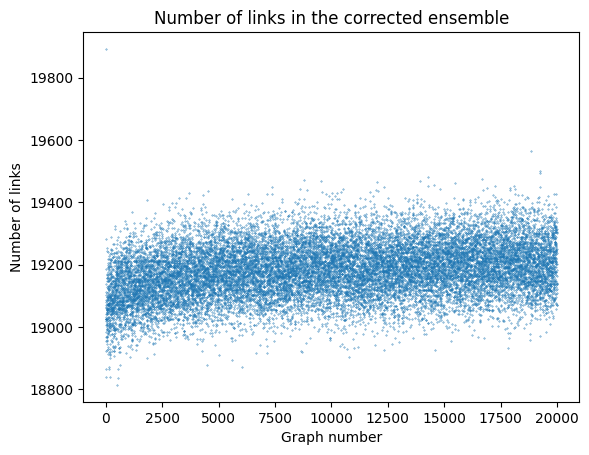
\includegraphics[scale=0.8]{../img/metropolis/num_links.png}
    \caption{Number of edges of each graph in the sampled ensemble, as the sampling went in time. We can see that in the beginning, the number of edges increases fast, therefore we should use a burn-in period.}
    \label{fig:num_links_MH}
\end{figure}

Secondly, to study if our sampling method reaches the highly probable states, we might take a closer look at some bias we might have introduced. The sample we start the algorithm with is a one where we connected nodes in a circle (node 1 to node 2 etc.) and we can thus study, how many of these edges stay retained after some period of sampling. We expect that the highly improbable edges vanish very quickly. If the number of retained edges reaches some steady state, we might say we reached some sort of equilibrium. 

The result can be seen on figure \ref*{fig:second_diagonal}. The number of preserved edges drops very quickly, but seems to be slightly decreasing even after $10\mathpunct{}000$-th sample. This also suggests, that to reach equilibrium, we would need much longer sampling. 

\begin{figure}[!ht]
    \centering
    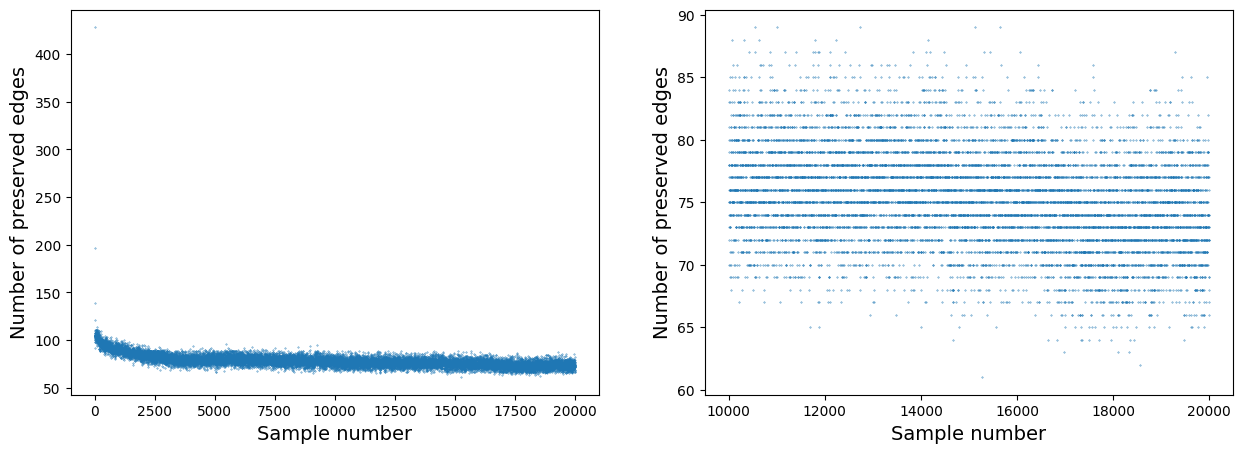
\includegraphics[scale=0.5]{../img/metropolis/second_diagonal.png}
    \caption{Number of edges on the ``second diagonal'' (i.e. $a_{12}, a_{23}, a_{34}$ and so on) which are retained during the sampling. Our initial sample connects edge 1 to 2, 2 to 3, ..., 1021 to 1, so initially there were 1021 such edges. After few samples, the number drops significantly and seem to decrease even after many samples. On the left we show the whole sampling procedure, on the right figure only after $10\mathpunct{}000$-th sample.}
    \label{fig:second_diagonal}
\end{figure}

Next, we are supposed to assign weights, for which we need the estimates of marginal probabilities for every edge. For that, we take samples from the $10\mathpunct{}000$-th on and compute the average adjacency matrix of these samples. Its entries are then the estimates of marginal probabilities. 

Similar to the original model, we can study if strengths were assigned well by comparing them with the empirical strengths. Figure \ref*{fig:degrees_strengths_corrected} shows that strengths are reproduced well for nodes with high empirical strengths, however, the nodes with lower empirical strengths have on average lower than demanded strength in the ensemble. Let us recall, that in case of Out-degree corrected SIM, we got perfect reconstruction (figure \ref*{fig:degrees_strengths_rec_corrected_naive}). There, we computed the marginal probabilities analytically, here, on the other hand, we had to use an estimate given by the average adjacency matrix. This can lead in underestimation of strengths in the region of low empirical strengths. 

The graphs to the left on the figure \ref*{fig:degrees_strengths_corrected} show the comparison of degrees. Here we see that indeed, both in- and out-degrees are corrected and reproduced better, unlike in the situation, where we only corrected out-degrees (figure \ref*{fig:degrees_strengths_rec_corrected_naive})
\begin{figure}[!ht]
    \centering
    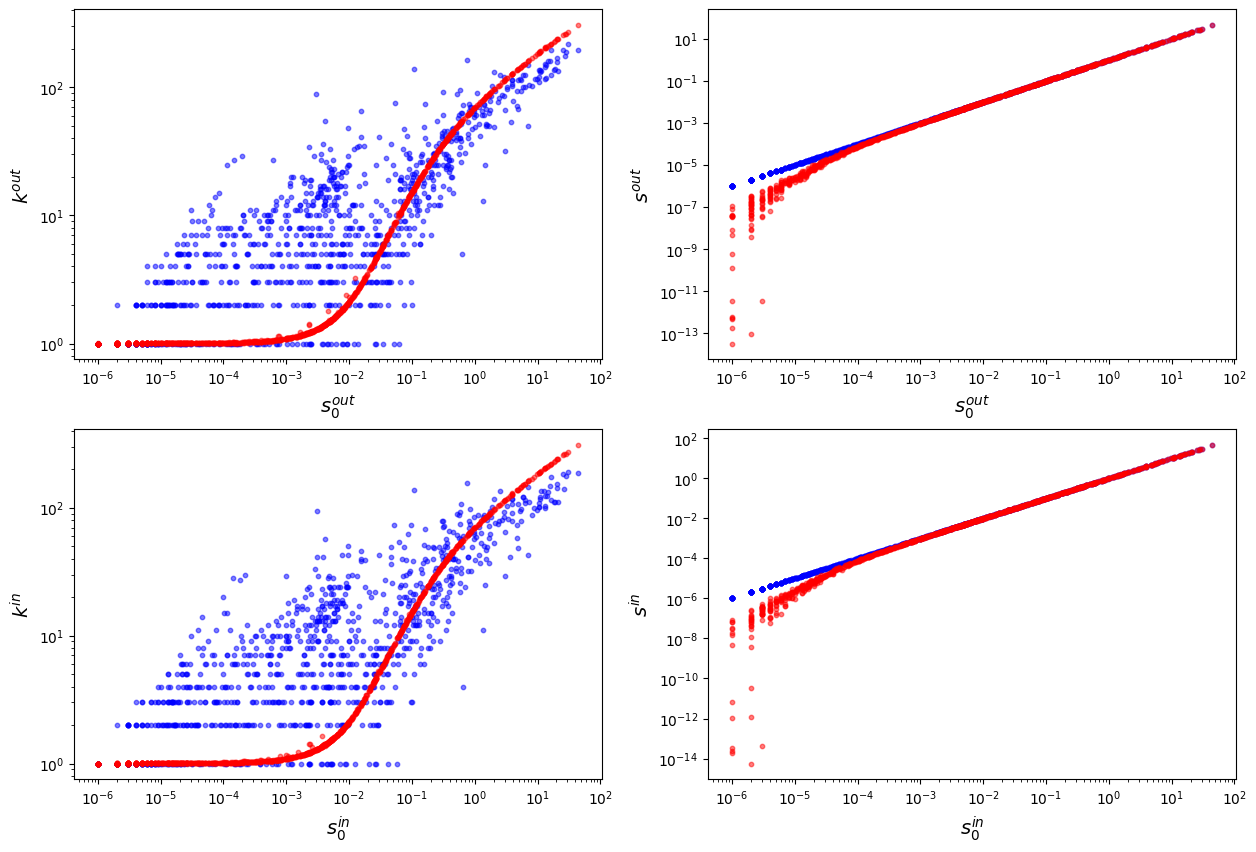
\includegraphics[scale=0.5]{../img/corrected/degrees_strengths_rec.png}
    \caption{Comparison similar to one on figures \ref{fig:deg_strengths_rec} and \ref*{fig:degrees_strengths_rec_corrected_naive}, but this time for the Degree corrected SIM.}
    \label{fig:degrees_strengths_corrected}
\end{figure}

Similarly to the original SIM, we may compare the histograms of degrees and strengths. Figure \ref*{fig:degrees_strengths_hist_corrected} shows for the degrees very similar results to those of the original SIM, apart from the case $k=1$. On the other hand, the results for strengths are very much different. Our degree-corrected model started producing nodes with much smaller strengths than which were observed in the empirical graph. Further investigation would be needed to show, whether it is due to limited size of the ensemble or it is a property of the model.

\begin{figure}[!ht]
    \centering
    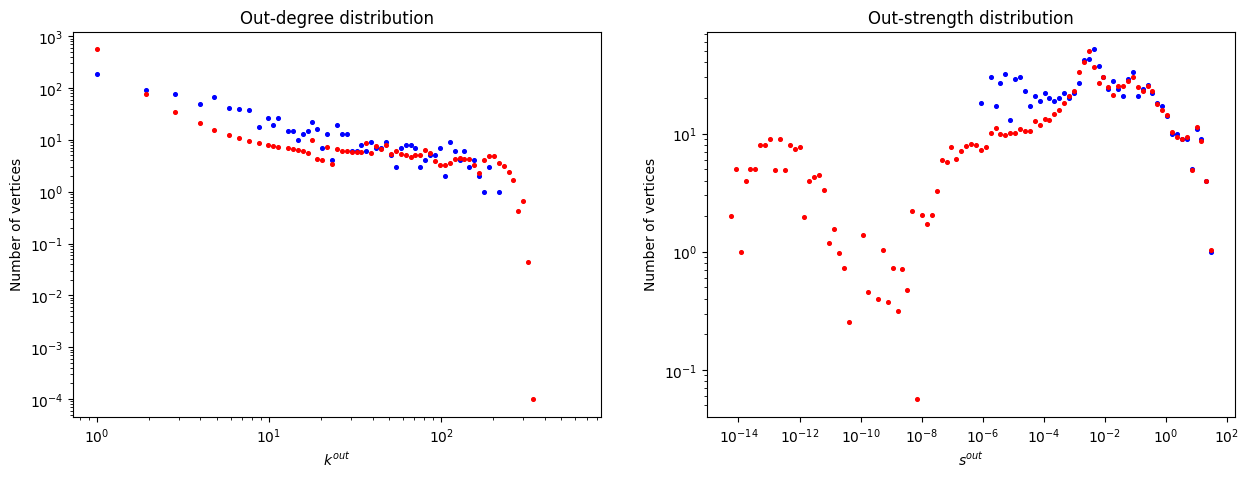
\includegraphics[scale=0.5]{../img/corrected/degrees_strengths_hist.png}
    \caption{Comparison of degree and strength histograms of the empirical graph and degree-corrected ensemble. }
    \label{fig:degrees_strengths_hist_corrected}
\end{figure}

We shall study the second order properties as well. First, let us focus on the ANND and ANNS (figure \ref*{fig:ANND_ANNS_corrected}). Compared to the original SIM (\ref*{fig:ANND_ANNS}), most of the nodes seem to follow similar pattern as in the original model, however, some of them start to manifest lowered ANND and ANNS. We investigated such nodes and found out, that they usually still keep their neighbor from the circle initialization of our sampling. We see that the problem is the more pronounced, the lower the empirical-strengths are. That is because in the Metropolis Hastings algorithm, it takes very long time for these nodes to obtain any other than the edge from the initialization, since any such edge is highly improbable. This could be solved by either waiting long enough or finding a better way to initialize the network. This just shows that even though the Metropolis-Hastings algorithm yields samples from the demanded distribution in the limit, it might actually take very long to truly replicate the distribution by sampling.

\begin{figure}[!ht]
    \centering
    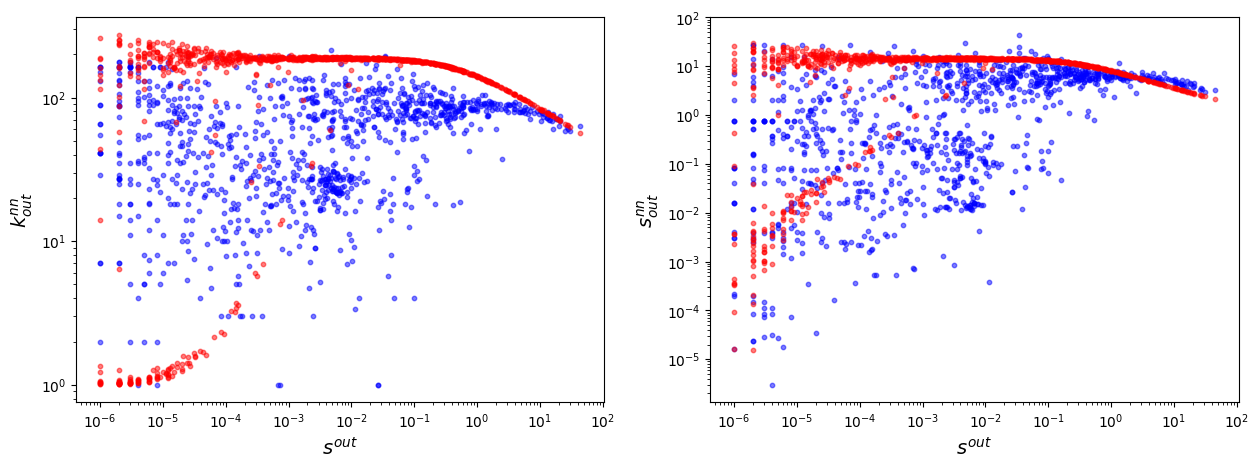
\includegraphics[scale=0.5]{../img/corrected/annd_anns.png}
    \caption{Comparison of ANND and ANNS for the original graph and its ensemble reconstruction using the Degree-corrected SIM. Compare with the original SIM (figure \ref*{fig:ANND_ANNS})}
    \label{fig:ANND_ANNS_corrected}
\end{figure}

Finally, we also show the aggregated version of ANND and local clustering coefficient for all nodes with the same degree (figure \ref*{fig:ANND_k_cl_coeff_k}, compare with figures \ref*{fig:ANND_k} and \ref*{fig:cl_coeff}). Compared with the original SIM, we notice only minor differences (with significant jump for $k=1$).

\begin{figure}[!ht]
    \centering
    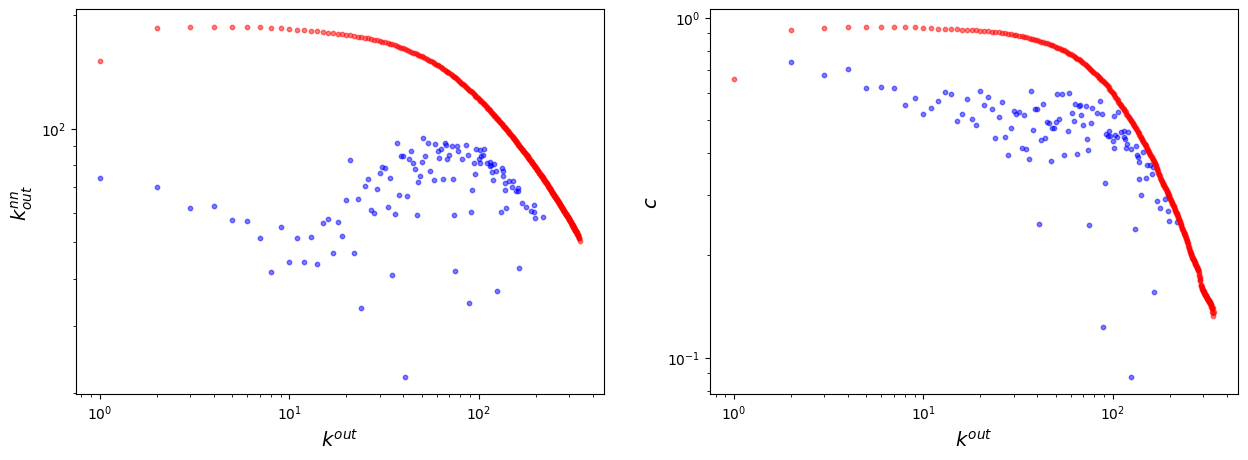
\includegraphics[scale=0.5]{../img/corrected/annd_k_cl_coeff_k.png}
    \caption{ANND and the local clustering coefficient, averaged for all nodes with the same degree (empirical network blue, ensemble reconstruction red). Compare with figures \ref*{fig:ANND_k} and \ref*{fig:cl_coeff}}
    \label{fig:ANND_k_cl_coeff_k}
\end{figure}

We might therefore conclude, that we obtained such a modification of the SIM, which achieved the nonzero degrees for each node while changing the other properties only in a very minor way. This is a good sign on one hand, on the other hand we might have hoped, that having the nonzero degrees would for example solve the problem of poor ANND reconstruction. We shall, however also remind ourselves, that we do not aim for a model applicable to all real-world networks, we only try to find models which are more or less suitable for specific domains. Even though some properties were not reproduced well enough for the airport network, it does not mean they would not be reproduced well for the financial network.